\documentclass[12pt]{article}

\usepackage[margin=1in]{geometry}
\usepackage{amsmath,amsthm,amssymb}
\usepackage[section]{placeins}
\usepackage{graphicx}
\usepackage{verbatim}
\usepackage[table,xcdraw]{xcolor}
\usepackage{subcaption}
\usepackage{listings}
\usepackage{booktabs}
\usepackage{setspace}
\newcommand{\N}{\mathbb{N}}
\newcommand{\Z}{\mathbb{Z}}
\newcommand{\C}{\mathbb{C}}
\newcommand{\R}{\mathbb{R}}
\newcommand{\Q}{\mathbb{Q}}
\newcommand{\E}{\mathbb{E}}
\newcommand{\Prob}{\mathbb{P}}
\newcommand{\lb}{\lbrace}
\newcommand{\rb}{\rbrace}
\usepackage{algorithm}
\usepackage[noend]{algpseudocode}


\lstset{
language=Python,
basicstyle=\scriptsize\ttfamily,
commentstyle=\ttfamily\color{gray},
numbers=left,
numberstyle=\ttfamily\color{gray}\footnotesize,
stepnumber=1,
numbersep=5pt,
backgroundcolor=\color{white},
showspaces=false,
showstringspaces=false,
showtabs=false,
frame=single,
tabsize=2,
captionpos=b,
breaklines=true,
breakatwhitespace=false,
title={Unsupervised Learning of Twitter Language Growth},
escapeinside={},
keywordstyle={},
morekeywords={}
}

\makeatletter
\def\BState{\State\hskip-\ALG@thistlm}
\makeatother

\linespread{1.5}

\newenvironment{theorem}[2][Theorem]{\begin{trivlist}
\item[\hskip \labelsep {\bfseries #1}\hskip \labelsep {\bfseries #2.}]}{\end{trivlist}}
\newenvironment{lemma}[2][Lemma]{\begin{trivlist}
\item[\hskip \labelsep {\bfseries #1}\hskip \labelsep {\bfseries #2.}]}{\end{trivlist}}
\newenvironment{definition}[2][Definition]{\begin{trivlist}
\item[\hskip \labelsep {\bfseries #1}\hskip \labelsep {\bfseries #2.}]}{\end{trivlist}}
\newenvironment{exercise}[2][Exercise]{\begin{trivlist}
\item[\hskip \labelsep {\bfseries #1}\hskip \labelsep {\bfseries #2.}]}{\end{trivlist}}
\newenvironment{problem}[2][Problem]{\begin{trivlist}
\item[\hskip \labelsep {\bfseries #1}\hskip \labelsep {\bfseries #2.}]}{\end{trivlist}}
\newenvironment{question}[2][Question]{\begin{trivlist}
\item[\hskip \labelsep {\bfseries #1}\hskip \labelsep {\bfseries #2.}]}{\end{trivlist}}
\newenvironment{corollary}[2][Corollary]{\begin{trivlist}
\item[\hskip \labelsep {\bfseries #1}\hskip \labelsep {\bfseries #2.}]}{\end{trivlist}}
\newenvironment{claim}[2][Claim]{\begin{trivlist}
\item[\hskip \labelsep {\bfseries #1}\hskip \labelsep {\bfseries #2.}]}{\end{trivlist}}

\title{Unsupervised Learning of Language Growth on Twitter}
\author{Arun Shanmuganathan}
\date{Supervisors: Dr. Scott Hale (OII) and Dr. James Martin (Stats)}
\begin{document}

\begin{titlepage}
    \begin{center}
        \vspace*{0.5cm}

        \Huge
        \textbf{Unsupervised Learning of Language Growth on Twitter}
        \vspace{0.5cm}

\LARGE Arun Shanmuganathan\\
        Jesus College\\

        \vspace{1.2cm}
        
\includegraphics[width=0.5\textwidth]{images/logo.png}
        \vspace{0.8cm}

\normalsize A dissertation submitted in partial fulfilment of the requirements for the degree of \\ Master of Science in Applied Statistics\\



        \vspace{0.8cm}



        \large
        Department of Statistics\\
        University of Oxford\\
        September 2017
    \end{center}
\end{titlepage}


\pagenumbering{arabic}

\begin{center}
\vspace*{2cm}
\textbf{\LARGE Abstract}
\end{center}
 \large This dissertation looks at the growth of language usage on Twitter from 2011 to 2017. It attempts to understand the way that different languages grow using the unsupervised machine learning techniques of clustering \& hidden Markov models with the aim of understanding how these trends differ across languages and the effect of short-term surges.
\\\\
It comes to 3 key conclusions:
\begin{enumerate}
\item There is  clear long-term impact of short-term surges on some languages (English, Japanese, Portuguese, Turkish \& French) but not for most languages.
\item There isn't a clear relationship between bilingual usage and long-term growth patterns but other growth similarities do exist.
\item English is a poor proxy for understanding language growth but better for larger languages than smaller ones.
\end{enumerate}
 \newpage

\begin{center}
\vspace*{2cm}
\textbf{\LARGE Acknowledgements}
\end{center}
 \large I am incredibly grateful to Dr Scott Hale for his generous support, ideas, time and enthusiasm for this project and my learning in general. I couldn't have done it without such a supportive and engaged mentor.
 \\\\
 I'm also extremely thankful to Dr James Martin who was my supervisor throughout the year, supporting me in a number of ways including making this project possible.
 \\\\
 Finally, to my parents who have been there through everything in my life and education - thank you so much.
 \newpage

\tableofcontents

\newpage

\section{Introduction}

\subsection{Motivation and Objectives}
Twitter is a social network platform launched in 2006 that allows individuals to publish 140 character posts known as 'tweets' to their direct network and a wider audience. It has since been built into a community of over 300 million active users from around the world. Headquartered in San Francisco, initial users used it almost exclusively in English but it has now grown so that the user interface of the platform is available in 42 languages and less than 50\% \cite{Halemain} of daily posts are in English now.
\\\\
It is common for communities using a single language to develop \cite{Halemain} but there is a process for a language to go from being non-existent on Twitter to being used by a thriving community . Given that bilinguals have been shown to play crucial roles in bridging these communities \cite{Halemain}, we speculate that this process involves bilinguals choosing initially to use a more popular language and then switching to using the less-common language and over time, more  users choosing to directly use their native language.
\\\\
The main aim of this study is to model this growth progression of languages on Twitter using a variety of unsupervised machine learning techniques to test three key hypotheses:
\begin{itemize}
\item Short-term surges can have long-term impacts on language growth.
\item There are similarities in growth patterns among languages that have similar levels of bilingual use (e.g. similarities between Japanese and Korean or between Filipino and Italian)
\item English is often a poor proxy to use when trying to understand community growth on Twitter
\end{itemize}
\subsection{Dissertation Structure}
The dissertation is divided into 6 main sections. Section 2 looks at the previous literature summarising the main conclusions and seeing how they lead to the questions that we ask in this study. Section 3 explains what data we have to work with, how we work with it and some problems. Section 4 gives a high level overview of the data through a number of exploratory methods. Section 6 attempts to cluster the data for specific languages including both K-means \& Agglomerative Hierarchical Clustering. Section 5 then attempts to model the data using a hidden Markov model with the Baum-Welch Algorithm. Section 7 then explicitly aims to answer our key hypotheses.
\newpage
\section{Relevant Past Work}
 Research interest in Twitter Language Communities has been trending over the fast few years \cite{Delia, Eleta, Garcia, geographies, Goncalves, Gonzalez, Graham, Hecht, Kim, Kwak, Poblete} but only recently has there been research investigating the differences between different languages \cite{Halemain, Hong, Nguyen2}. These recent studies have confirmed the amount of language-based division on Twitter. The connectivity of these languages is looked at further as a social network attempting to understand the interplay between languages and how communities connect \cite{Halemain}. One of the key conclusions that underpin this research is the importance of bilinguals in bridging these communities. In this study, it was found that multilingual users played a crucial role in bridging communities with the vast majority of users only retweeting in the same languages as their own. With the aim of understanding this better, we look to what the growth trends have been and how they may have caused these relationships between language communities. Because languages need to grow from non-existence to relevance over an extended period of time, we suspect that in their initial growth, these bilingual users have an even more important role to play in the development of these languages over time.
\\\\ The research also shows that language users in some communities have operated similarly in terms of the levels of crossover to other languages as well as commonality in hashtags, URLs, connections \cite{Hong} and bilingual use. In particular, it was found that there was an Asian-language group (Japanese, Korean and Thai) that had relatively closely connected communities (more crossover than expected given their relative lack of multilingual users) as well as a similarity in the way that Italian and Filipino users were very willing to cross over and use other languages. We extend this further to see which languages are similar in terms of their growth patterns and moreover, which sets of languages differ substantially in their growth from other languages. We specifically look at this in trying to find whether there are any noticeable similarities to the previous research between pairs of communities.\\\\
The vast majority of studies in the past have only looked at English language conversations on Twitter \cite{HechtEnglish} and it has recently been shown that there are some reasons, regarding the way that different language communities use Twitter, that we should be skeptical of this approach and maybe consider alternatives \cite{Garcia, Halemain, Hong}. We look at this in greater depth directly questioning this assumption with the goal of also finding which languages English does act as a good proxy for in the realm of language growth.\\\\
Despite many studies being conducted using Twitter language data, this is the first, to our knowledge, that looks into the change over time of these language communities. Research has been done on how conversations and political movements grow on Twitter \cite{HMM, Gonzalez} and this study uses some of the techniques used as a basis in terms of the underlying models, particularly looking at growth rates and the relevance of friend-follower relationships \cite{Gonzalez}, which have previously shown to have relevance in the growth of movements concluding that growth of movements should be seen as macro diffusion processes rather than individual binary decision making. We use this approach in our study looking at a large collection of users and changes of the macro-group rather than looking at individual bilingual users. \\\\
The use of unsupervised learning techniques for Twitter data has grown with a number of studies using various clustering techniques to classify users based on how they interact and engage \cite{Goncalves}  as well as understanding conversations with sentiment analysis \cite{HMM}. We extend this further to use the incredibly clear time-series data that comes from the structure of data to create Hidden Markov Models as well as a variety of clustering techniques. Studies have also been done into time-series and using unsupervised techniques to understand the progressions of these time series \cite{Oates} and we look into applying these methods to the time series that we extract.

\newpage
\section{Data}
\subsection{Available Data}
Using Twitter's Spritzer access, we have access to data on a representative sample of all posts from 28th September 2011 to 1st January 2017 (with some notable gaps discussed later). The documentation for this used to say that this was approximately 1\% of all posts on Twitter but this is no longer the case. We work with the following primary variables on each post:\\\\
$id$ - The post's ID number\\
$created\_at$ - The time the post was created\\
$user$:$followers\_count$ - No. of followers of the user at the time of the post\\
$user$:$friends\_count$ - No. of friends of the user at the time of the post\\\\
We then process this using Hive to get daily summaries for each language. The secondary variables for each day/language pair are:\\\\
$posts$ - the total number of posts representing activity\\
$followers$ - the total number of followers of users that made those posts representing  reach/sum of the out-degrees\\
$friends$ - the total number of friends of users that made those posts representing existing community influence/sum of the in-degrees\\\\
We note here that for the followers and friends variables, we on many occasions will be counting some users multiple times if they posted more than once in the same day. This is appropriate because we want each of those posts to represent more activity/reach/influence. If we were to count it per user, we wouldn't get the total reach of all posts in that time period.\\\\
Initially, we extracted the data in hourly summaries but we find that a significant problem occurs in that different languages are more or less common at different times of the day. We take different attempts to solve for this including taking it with respect to a baseline average activity over multiple days but we find that none of these are to our satisfaction and that there is enough data to work on this from a purely aggregate daily level. We find that accounting for the weekend is unnecessary, which we look into later.

\subsection{Language Detection}
Due to the lack of language data of posts from 2011 to the end of 2012, we wish to get a more complete data set, especially since many languages were just beginning to grow during this time. As a result, we use the Compact Language Detection (CLD) kit version 2 \cite{CLD}, which is used in language detection in Google Chrome too, and which Graham et all (2014) \cite{Graham} found performed fairly well on Twitter content. We also use the recommendations [3] of removing URLs and user names from the text of posts before performing language detection. We only use data ,that the CLD reports the language identified as reliable, and for which more than 50\% of the post is in the particular language. This is to ensure that we are confident of the language detection and that it doesn't consist of a 'bilingual post', which may be of interest but is outside the scope of this study. The language detection kit was able to detect the language of 82.68\% of all 6,501,496,268 available posts during the time reliable and of those 5,375,308,805, just 0.04\% of them (2,386,017) didn't have one language more than 50\% of the post. This left us with 5,372,922,788 tweets to work with.
\subsection{Missing Data}
We do have some clear points of missing data especially in late 2011, early 2014, early 2015 and late 2015. This is due to the published data not being available for this time. We check for other trends of missing data e.g. missing certain languages or missing at certain time periods of the day and find that there there are no significant outliers or trends of the days that have missing data. In order to account for these missing periods, we simply make sure when looking at growth to ensure that we take out the starts of these periods. This definitely limits the scope of the study but we still have quite a lot of data that should explain enough of what we want.
\\\\
The full list of missing dates included 186 days with particularly long stretches in the following times: 30/11/11 - 31/12/12 (32 days), 02/01/14-04/02/14 (34 days), 02/01/15-21/03/15 (78 days) and 23/11/15-14/12/15 (22 days) with only 20 random other days of missing data. Given that our data set is a full 1737 days in total, we still have enough data to proceed with the analysis.
\newpage

\section{Exploratory Data Analysis}
\subsection{Static Summary}
We initially look at the data in a static sense and find some simple summary statistics over entire time period in the most common languages as shown in Table 1.
\FloatBarrier
\begin{table}[htbp]
\begin{center}
\caption{Summary of 14 most commonly used languages}
\begin{tabular}{lrrrrr}
\toprule
Language & posts &  Pcg. posts (\%) & Foll/post   & Friend/post &  Friend/Foll Ratio  \\
\midrule
en   &  2212375146 &       41.18 &     2876 &       1057 &               2.72 \\
ja   &  1010740298 &       18.81 &      767 &        583 &               1.32 \\
es   &   547196732 &       10.18 &     4784 &       1044 &               4.58 \\
ar   &   305418519 &        5.68 &     6432 &       3710 &               1.73 \\
pt   &   292656979 &        5.45 &     2535 &        948 &               2.67 \\
ms   &   277611219 &        5.17 &     2663 &        449 &               5.94 \\
ko   &   113170646 &        2.11 &      725 &        546 &               1.33 \\
tr   &   108612421 &        2.02 &     3970 &       2237 &               1.78 \\
th   &    96421055 &        1.79 &      634 &        283 &               2.24 \\
fr   &    92452723 &        1.72 &     1811 &        690 &               2.63 \\
ru   &    88552043 &        1.65 &     1219 &        472 &               2.58 \\
nl   &    33353729 &        0.62 &     1034 &        391 &               2.65 \\
tl   &    30630768 &        0.57 &     1560 &        449 &               3.47 \\
it   &    29218953 &        0.54 &     2640 &       1047 &               2.52 \\
\bottomrule
\bottomrule
\end{tabular}
\end{center}
\end{table}
\FloatBarrier
The languages in Table 1 represent the top 14 languages in terms of post proportion, which represents a good cutoff as there is a significant drop-off to less than half the number of posts after this cutoff. We also merge the Indonesian (id) and Malay (ms) languages because their linguistic similarity results on language detection challenges [1]. For the rest of this study, we will simply refer to Malay but include Indonesian. It is important that in this table and for future analysis, the object of interest is the post itself and when looking at the follower, friend and status count - we look at the respective count of the user who wrote that post and we associate it with the post. The interpretation of this is that e.g. on average, each English post was on average reached by 2876 followers, influenced by 1057 friends and was reached by 2.72 people for every person it was influenced by.\\
We already note some interesting features related to previous work:
\begin{itemize}
\item A comparison to a language determination study in 2010 [7] shows that Spanish and Arabic have grown relatively rapidly whilst English and Portuguese declining in relative popularity.
\item Japanese, Korean and Thai have relatively few of both followers and friends per post suggesting that users of these language aren't as connected as others. It is interesting to note that these languages were found to be in a similar cluster of Asian languages [1] and that they were 3 of the top 4 most languages in terms of insularity (i.e. languages whose speakers did not interact with content in other languages)
\item The other language that was found to be particularly insular was Turkish exhibits the opposite in that both friend and follower per post are relatively high. This is quite similar to Arabic which may suggest something about it's usage in the Middle East.
\item The posts in Malay, Spanish and Filipino seem to be more dominated by 'influencers' - i.e. people that have significantly more followers than friends.
\end{itemize}
\subsection{Initial Timeseries}
We first look at the 6 most common languages over time and see their growth in post rate over time. Note that we can only look at proportional growth (i.e. how the relative proportion of each language changes over time) because Twitter has changed the percentage of posts it includes within the sample 'Spritzer' stream over the years and these changes are not well documented. The stream provides a small random sample, which used to be approximately 1\% of all posts but this figure is no longer included in the documentation. This gives us Figure 1 below:
\FloatBarrier
\begin{figure}[hbtp]\centering
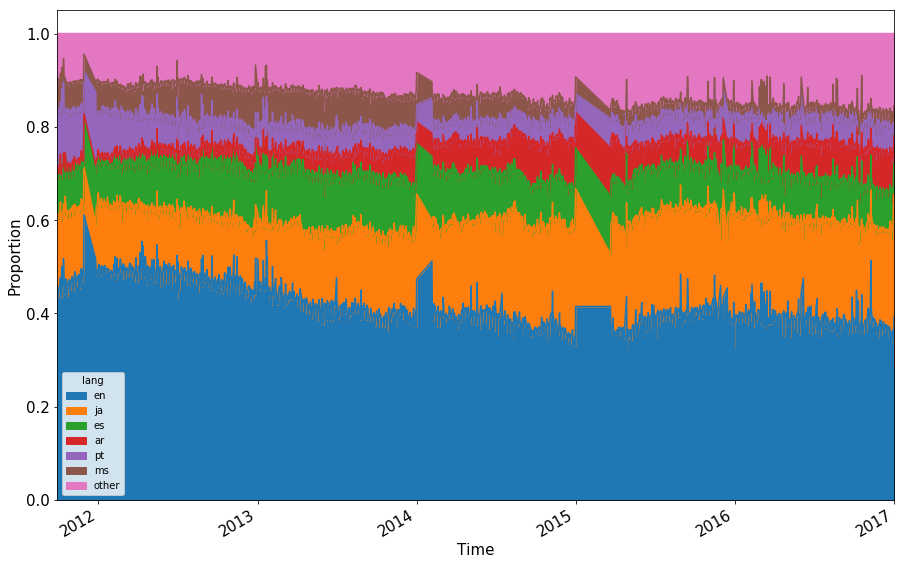
\includegraphics[width=\textwidth,clip]{images/languageproportionplot.png}
\end{figure}
\FloatBarrier
This explains more clearly the earlier finding of the growth of Arabic and the decline of English and Portuguese while suggesting that the growth of Spanish may have happened before this. The decline of Malaysian/Indonesian is also made apparent. It also highlights some of the problems with the data in that there is no data in the periods mentioned earlier and so has just interpolated between points. The presence of spikes is what we hope to look for the effect of when we define 'surges' and see if this results in long-term impact.
\subsection{Language Correlations}
We want to look further and see the relationships between languages and whether some languages grow at the expense of others or grow together. To that extent, we create a heat map on the correlation matrix between daily post proportions of languages.
\FloatBarrier
\begin{figure}[hbtp]\centering
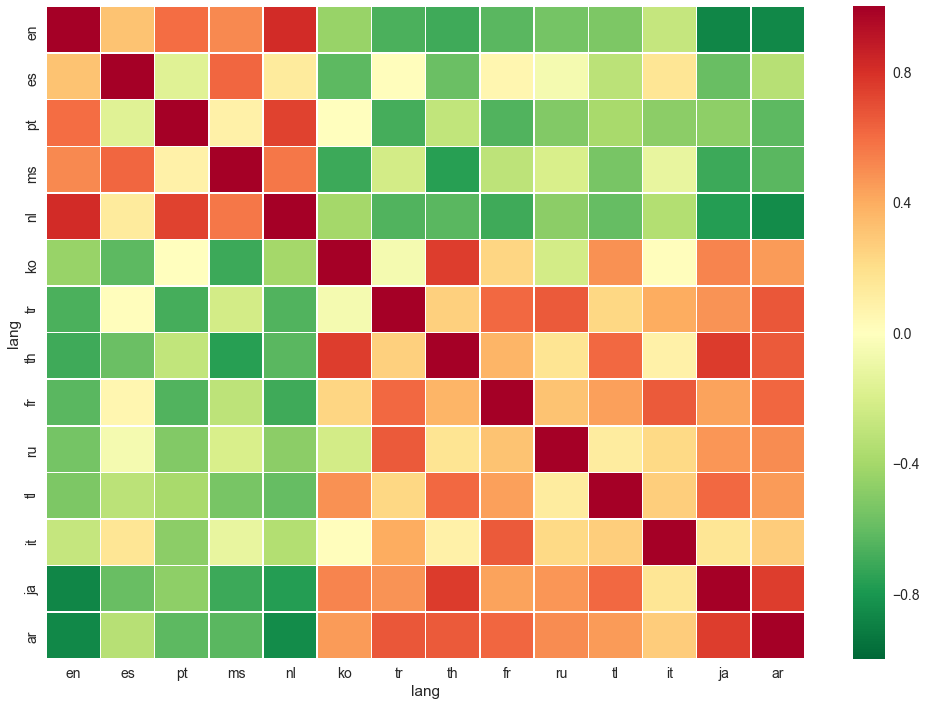
\includegraphics[width=0.9\textwidth,clip]{images/correlation.png}
\end{figure}
\FloatBarrier
By simply putting them such that all the languages positively correlated with English are on the left and all the ones negatively correlated are on the right, we end up with the heat map that very clearly shows a division between the sets of languages where they are correlated to others in the same group and negatively correlated to the others with few exceptions. This isn't very surprising given that we're looking at proportions and so growth is measured zero-sum i.e. growth of somethings have to come at the expense of others but it's surprising how well classified these groups are. Future work should explore in more detail some of the exceptional pairs e.g. (Italian-Spanish, Korean-Russian) as well as some of the more extreme correlations (Thai-Japanese, Dutch-Arabic).
\subsection{Measurements of Growth}
From this, we notice trends in growth and some relationships between languages but in order to have a more quantitative study using unsupervised techniques we need clear measures of growth. \\\\
Currently, our data consists of points $x_{i,j,t,}$ for $j=1\ldots J$, the languages, $t=0 \ldots T$, time (in days) and $i=1,2,3$ where $i=1$ refers to the number of posts, $i=2$ refers to the number of followers and $i=3$ refers to the number of friends. In order to account for the different amounts of data in each given day, we instead use the proportions: $$p_{i,j,t} = \frac{x_{i,j,t}}{\sum_{j=1}^{J} x_{i,j,t}} \forall i,j,t$$ such that $\sum_{j=1}^{J} p_{i,j,t} = 1 \forall i,t$. The reason for normalising the post rate is clear and the reason for normalising the other two values is to ensure that we're measuring like-for-like. If we were to not normalise, we would still run into the problem that we're not sure how much these are affected by surges and declines at any given time but normalising ensures this. \\\\
When we measure growth, we normally look at relative gains from a previous baseline. For this study, we simply look at the previous baseline as the previous day. I.e. the growth figures we look at are:
$$ q_{i,j,t} = \frac{p_{i,j,t} - p_{i,j,t-1}}{p_{i,j,t-1}} \forall i,j,t$$ for $i=1,2,3, j = 1 \ldots J$ and $T=1,\ldots T$. We could have taken the gains relative to some moving average in order to smooth out the results but this approach more clearly reflects how each daily movement is dependent on the previous day's movement and the results are already fairly smooth. We could also have adjusted for weekends but there was no noticeable effect and to do so would have involved looking at different time zones and different weekends around the world (e.g. Thursday and Friday in some parts of the Muslim world and Friday and Saturday in others \cite{Weekends}).
\FloatBarrier
\begin{figure}[hbtp]\centering
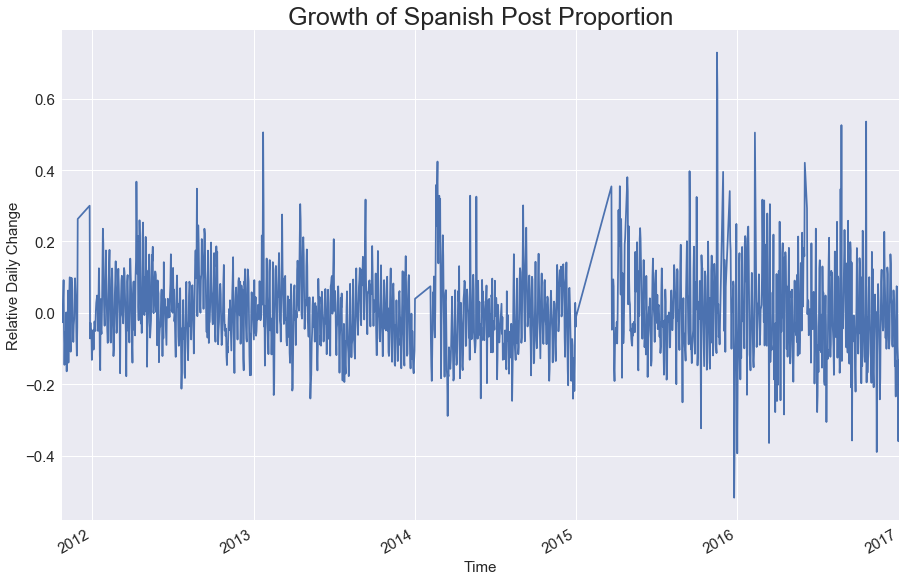
\includegraphics[width=\textwidth,clip]{images/SpanishProportionGrowth.png}
\end{figure}
\FloatBarrier
\newpage
\section{Clustering}
Now that we have the measures of growth for each day/language pair, we wish to classify each day into a period of either decline, stability, growth or surge for each language. Our argument for choosing these 4 periods is both from our earlier visualisations of growth proportions, tests on the data using differing number of periods as well as from previous studies on agent-based models of language competition \cite{competition, competition2, competition3}.
\subsection{K-means Clustering}
We initially try out a simple k-means clustering of points, where each point has 3 dimensions and we look only at the points for a specific language. The goal here is for each language, to label each day as either 0,1,2 or 3 representing our decline, stability, growth and surge respectively. In K-means clustering, the goal is to minimise the sum of distances that each point is away from the centroid of points with those labels. I.e. Given $c_t$ for each $t=1 \ldots T$ where $c_t$ takes values in $0,1,2,3$, we get centroids $\mu_0,\mu_1,\mu_2,\mu_3$ of the set of points with $k=0,1,2,3$ respectively. Then after that, we get our overall distance which is the sum of the $\lVert q_t - \mu_k \rVert $ such that each $q_t$ is only counted once in the $k$ for which $c_t = k$. In particular, for clusters $C_0,C_1,C_2,C_3$ we aim to minimize: $$\sum_k\sum_{t \in C_k} \lVert q_t - \mu_k \rVert $$
\\
\FloatBarrier
\begin{algorithm}
\caption{K-Means Clustering}
\begin{algorithmic}[1]
\Procedure{Label each day for a given language as 0: Decline, 1: Stability, 2: Growth or 3: Surge}{}
\BState Randomly initialize $\mu_0, \mu_1, \mu_2,\mu_3$ as centroids.
\BState \textbf{for} t = 1 to T, \textbf{do}
\State $c_t \gets argmin_{k} \lVert q_t - \mu_k \rVert$
\BState \textbf{end for}
\BState \textbf{for} k = 0 to 3, \textbf{do}
\State $\mu_k \gets \frac{1}{\lvert \lbrace t\mbox{ : }c_t = k \rbrace \rvert} \sum_{c_t = k} q_t$
\BState \textbf{end for}
\BState $D \gets \sum_k \sum_{c_t = k} \lVert q_t - \mu_k \rVert $.
\BState Repeat steps 3 to 9 until D converges.
\BState Rotate labels such that $\lVert \mu_0 \rVert < \lVert \mu_1 \rVert < \lVert \mu_2 \rVert < \lvert \mu_3 \rVert$
\BState \textbf{Return} $\mu_0,\mu_1,\mu_2,\mu_3$ and $c_t \forall t$
\EndProcedure
\end{algorithmic}
\end{algorithm}
\FloatBarrier
As an example, we see the Arabic language data shown below as a histogram projected where we only look at a projection of the labels onto the activity and reach growth dimensions.
\FloatBarrier
\begin{figure}[hbtp]\centering
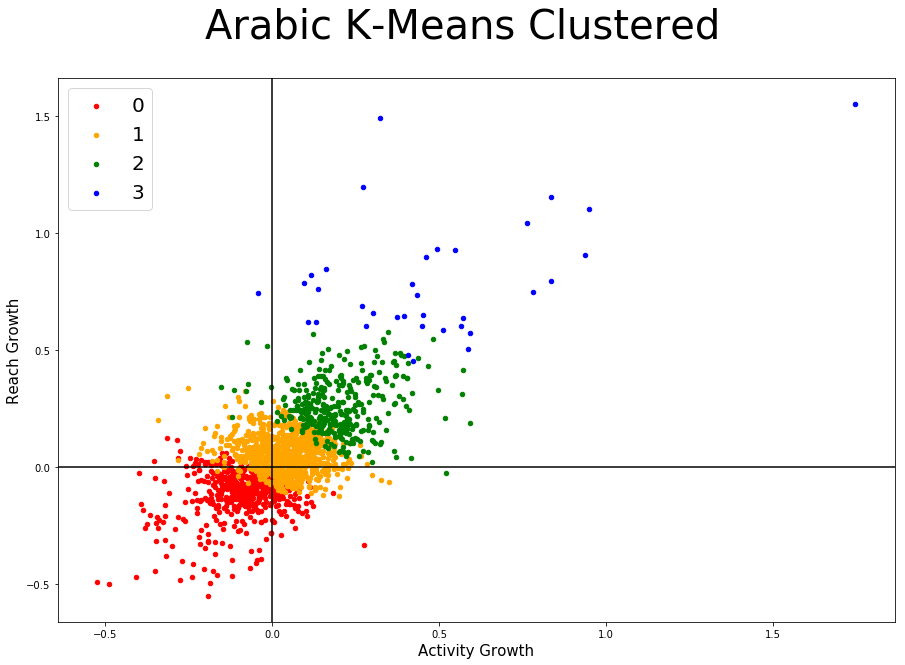
\includegraphics[width=0.78\textwidth,clip]{images/ArabicKMeans.png}
\end{figure}
\FloatBarrier
We can then turn this into an 'observed transition matrix' by looking at the frequency of switches between states as well as into a general probability distribution showing how often any given state occurs. These are shown below:
\begin{center}
\captionof{table}{K-means Clustered Distribution \& Transition Matrix of Arabic Progression}
\begin{tabular}{lr}
\toprule
Stage  & Probability \\
\midrule
Decline &  0.297 \\
Stability &  0.479 \\
Growth &  0.203 \\
Surge &  0.020 \\
\bottomrule
\end{tabular}
\quad
\begin{tabular}{lrrrr}
\toprule
Stage & Decline &  Stability & Growth & Surge \\
\midrule
Decline     &  0.613 &  0.314 &  0.061 &  0.012\\
Stability     &  0.195 &  0.628 &  0.165 &  0.012 \\
Growth     &  0.078 &  0.397 &  0.5 &  0.026 \\
Surge     &  0.286 &  0.2 &  0.229 &  0.286\\
\bottomrule
\end{tabular}
\end{center}
\vspace{0.5cm}
The transition matrix is shown such that a value on the $i$'th row and $j$'th row represents the probability of switching to stage $j$ given the previous day was on stage $i$ and as such the rows sum to 1. We notice some clear trends that seem fairly intuitive: the diagonals are fairly high meaning that they do stay in the same stages over consecutive days and there is a shift from surge to growth meaning that long-term impacts can occur form our surges.
\subsection{Agglomerative Hierarchical Clustering}
Now, we instead use a hierarchical clustering technique. In this, we start with 1 cluster for each point with the goal of combining clusters of minimum distance apart from each other until we remain with just 4 clusters. The distance we use between points is a simple Euclidean distance using the Ward's distance linkage method which aims to minimise the within-cluster variance total of the new set of clusters. When a cluster is just a single point, it takes the variance as the Euclidean-square distance of that point. In this method, for clusters $C_0,C_1,C_2,C_3$ we aim to minimise $$\sum_k \frac{1}{\lvert C_k \rvert}\sum_{t \in C_k} (q_t - \mu_k)^2$$\\
\FloatBarrier
\begin{algorithm}
\caption{Agglomerative Hierarchical Clustering}
\begin{algorithmic}[1]
\Procedure{Label each day for a given language as 0:Decline, 1:Stability, 2:Growth or 3:Surge}{}
\BState Initialise $T$ clusters for each $t=1$ to $T$
\BState $n \gets T$, the number of clusters
\BState \textbf{while} $n > 4$ \textbf{do}
\State \textbf{for} i,j = 1 to n \textbf{do}
\State $\indent M(i,j) = Var(C_i \cup C_j) - Var(C_i) - Var(C_j)$
\State \textbf{end for}
\State $(i^{\ast},j^{\ast}) =$ argmin $M(i,j)$
\State Merge clusters $i^{\ast}$ and $j^{\ast}$
\State Relabel clusters to be from $1$ to $n-1$
\BState \textbf{end while}
\BState Rotate labels such that the means are in order: $\lVert \mu_0 \rVert < \lVert \mu_1 \rVert < \lVert \mu_2 \rVert < \lvert \mu_3 \rVert$
\BState \textbf{Return} $C_0,C_1,C_2,C_3$
\EndProcedure
\end{algorithmic}
\end{algorithm}
\FloatBarrier
We again see the Arabic language data shown below as a histogram projected where we only look at a projection of the labels onto the activity and reach growth dimensions.
\FloatBarrier
\begin{figure}[hbtp]\centering
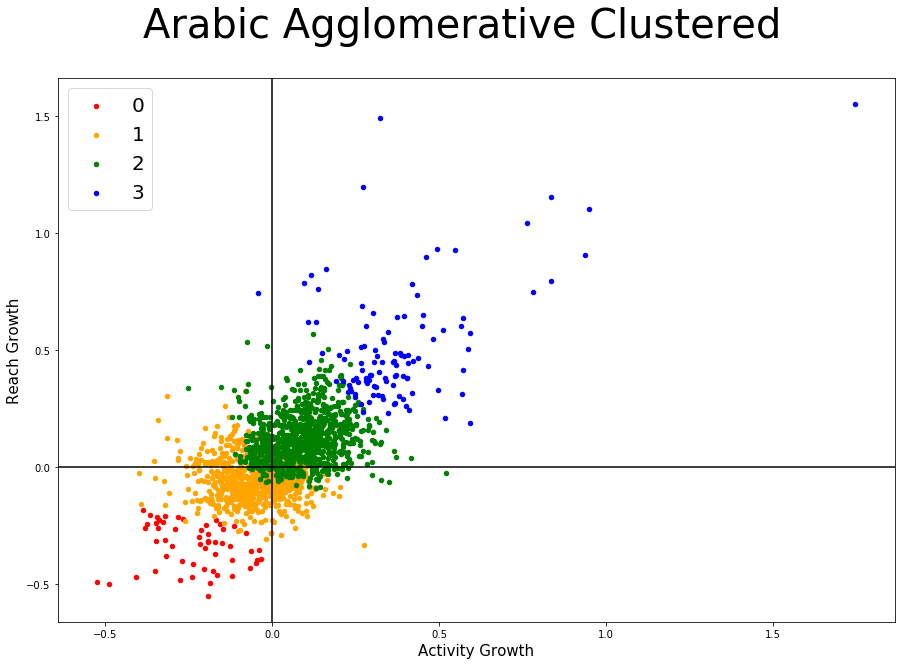
\includegraphics[width=0.72\textwidth,clip]{images/ArabicWardMethod.png}
\end{figure}
\FloatBarrier
We can then again turn this into an 'observed transition matrix' by looking at the frequency of switches between states as well as into a general probability distribution showing how often any given state occurs. These are shown in the figure below:
\begin{center}
\captionof{table}{Agglomerative Clustered Distribution \& Transition Matrix of Arabic Progression}
\begin{tabular}{lr}
\toprule
Stage  & Probability \\
\midrule
Decline &  0.033 \\
Stability &  0.402 \\
Growth &  0.501 \\
Surge &  0.064 \\
\bottomrule
\end{tabular}
\quad
\begin{tabular}{lrrrr}
\toprule
Stage & Decline &  Stability & Growth & Surge \\
\midrule
Decline   &  0.268 &  0.393 &  0.268 &  0.071 \\
Stability     &  0.039 &  0.652 &  0.281 &  0.028 \\
Surge     &  0.013 &  0.231 &  0.704 &  0.052 \\
Growth     &  0.027 &  0.181 &  0.409 &  0.382 \\
\bottomrule
\end{tabular}
\end{center}
\vspace{0.5cm}
We again notice the high diagonal and the even higher probability of switching from surge to growth and from decline to stability suggesting that this model gives higher weight to the stability and growth phases and not much chance of the decline \& surge stages.
When comparing these two models, we find that the K-means model better defines our interpretation of the 4 clusters because the origin, lies clearly within our second cluster and almost everything to the bottom of that lies in decline whereas in the agglomerative model, the origin lies in the 3rd cluster which contradicts our idea of 'growth'.
\newpage
\section{Hidden Markov Model}
\subsection{Definition \& Assumptions}
We now proceed to apply a Hidden Markov Model to our system. In a hidden Markov model $(X,Y)$, $X$ is a homogeneous Markov model which has $N$ different possible states. It has a starting probability $\mu$ and a transition matrix $A$ such that:
\begin{align*}
\mu_i &= \Prob(X_0=i)\\
A_{i,j} &= \Prob (X_{t+1} = j \vert X_t = i)\\
&= \Prob(X_{t+1} = j \vert X_0\ldots X_{t-1},X_t = i)
\end{align*}\\
where the second equality is known as the 'Markov Property' and defines a Markov Chain. In the Hidden Markov Model, the Markov Model is hidden and we only see our observed variables $Y$, which come from different distributions depending on the value of the corresponding hidden variable. I.e. there exist $N$ distributions $\phi_{1,\ldots N}$ such that $$ Y_t \vert X_t = n \sim \phi_n$$. \\The directional dependencies of the Hidden Markov Model are shown in the figure below.
\FloatBarrier
\begin{figure}[hbtp]\centering
\caption{Hidden Markov Model}
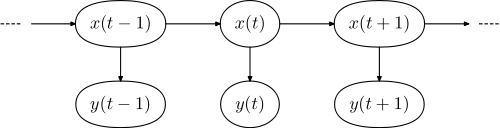
\includegraphics[width=\textwidth,clip]{images/MarkovChainExplanation.png}
\end{figure}
\FloatBarrier

In our particular Hidden Markov Model, we have exactly 4 states that our underlying Markov chain can take - again decline, stability, growth and surge. We need to work out 3 things in our model: the starting probabilities, the transition matrix and the emission functions.
\\
The assumptions underlying the Hidden Markov Model are that:
\begin{enumerate}
\item The underlying chain has the Markov Property - the reason this assumption is valid is because our growth figures are being determined from just the previous day and all previous growth is captured in the results of the previous day.
\item Homogeneity of the transition matrix (i.e. the transition matrix is independent of time) - this assumption is harder to justify but seems valid given the broad definitions of the stages that can apply at any time.
\item Time independence of the emission functions - this assumption is valid because of the way that we've defined the measures of growth to be scaled across any time.
\end{enumerate}

\subsection{Baum-Welch Algorithm}
In order to estimate our starting probabilities and transition matrix, we propose using the Baum-Welch algorithm learning from the given observations that we have for each language. The Baum-Welch algorithm aims to find the values of the unknown parameters using forward-backward recursion. It applies the Expectation-Maximization procedure to find the maximum likelihood estimate of the parameters given a set of observed features. The first step of this is the forward-algorithm. It takes in a series of observed values $y_1,\ldots y_t$ and computes $\alpha_i(t)$ the probability of being in state $i$ at time $t$ and seeing those observed values.
\\
\FloatBarrier
\begin{algorithm}
\caption{HMM Forward-Algorithm}
\begin{algorithmic}[1]
\Procedure{Compute $\alpha_i(t)$}{}
\BState \textbf{for} i = 1 to N, the number of states \textbf{do}
\State $\alpha_i(1) \gets \mu_i \phi_i(y_1)$
\BState \textbf{end for}
\BState \textbf{for} s = 1 to t-1 \textbf{do}
\State \textbf{for} i = 1 to N \textbf{do}
\State $\indent \alpha_i(s+1) \gets \phi_i(y_{s+1}) \sum_{i=1}^N \alpha_j(s)A_{i,j}$
\State \textbf{end for}
\BState \textbf{end for}
\BState \textbf{return} $\alpha$
\EndProcedure
\end{algorithmic}
\end{algorithm}
\FloatBarrier
The next step is the backwards-algorithm which takes in the end of a sequence $y_{t+1},\ldots y_T$ and computes $\beta_i(t)$, the probability of seeing those observed values given that you're in state $i$ at time $t$.\\
\FloatBarrier
\begin{algorithm}
\caption{HMM Backward-Algorithm}
\begin{algorithmic}[1]
\Procedure{Compute $\alpha_i(t)$}{}
\BState \textbf{for} i = 1 to N \textbf{do}
\State $\beta_i(T) \gets 1$
\BState \textbf{end for}
\BState \textbf{for} s = T-1 to t \textbf{do}
\State \textbf{for} i = 1 to N \textbf{do}
\State $\indent \beta_i(s) \gets \sum_{i=1}^N \beta_j(s+1)A_{i,j} \phi_j(y_{s+1}) $
\State \textbf{end for}
\BState \textbf{end for}
\BState \textbf{return} $\beta$
\EndProcedure
\end{algorithmic}
\end{algorithm}
\FloatBarrier
Now with these forward and backward recursion algorithms, we can use the expectation-maximisation procedure to determine the updating procedure in our unsupervised learning. First, we have our $\gamma$ function which is simply a combination of our forward \& backward algorithms to find the probability of being in state $i$ at a time $t$ given an observed sequence.
\begin{align*}
\gamma_i(t) &= \Prob (X_t = i \vert Y,A,\phi,\mu)\\
&= \frac{\Prob(X_t=i,Y \vert A,\phi,\mu)}{\Prob(Y\vert A,\phi,\mu)}\\
&= \frac{\alpha_i(t)\beta_i(t)}{\sum_{j=1}^N \alpha_j(t)\beta_j(t)}
\end{align*}
We can also get our joint marginal function $\epsilon$ which determines whether we are in states $i$ and $j$ at times $t$ and $t+1$ respectively.
\begin{align*}
\epsilon_{i,j}(t) &= \Prob (X_t = i,X_{t+1}=j\vert Y,A,\phi,\mu)\\
&= \frac{\Prob(X_t = i,X_{t+1}=j,Y \vert A,\phi,\mu)}{\Prob(Y\vert A,\phi,\mu)}\\
&= \frac{\alpha_i(t)A_{i,j}\beta_j(t+1)\phi_j(y_{t+1})}{\sum_{r=1}^N\sum_{s=1}^N \alpha_r(t)A_{r,s}\beta_s(t+1)\phi_s(y_{t+1})}
\end{align*}
\FloatBarrier
From these, we now update our parameters $\mu$ and $A$ to represent the new probabilities $\Prob(X_1 = i \vert Y)$ and $\Prob(X_{t+1} = j \vert X_{t} = i,Y)$
\begin{align*}
    \mu^{\ast} &= \gamma(1)\\
    A_{i,j}^{\ast} &= \frac{\sum_{t=1}^T\epsilon_{i,j}(t)}{\sum_{t=1}^T\gamma_i(t)}
\end{align*}
In the Baum-Welch algorithm, this is done repeatedly until the value of the likelihood of observing our $Y$ (given by $\sum_{j=1}^N \alpha_j(T)\beta_j(T)$) converges noting that this value increases in each iteration as a result of taking the maximum likelihood estimater of the parameters at each step.\\
\begin{algorithm}
\caption{HMM Baum-Welch Algorithm}
\begin{algorithmic}[1]
\Procedure{Optimize Transition Matrix and Starting Probability given Observations}{}
\BState \textbf{for} t = 1 to T \textbf{do}
\State \textbf{for} i = 1 to N \textbf{do}
\State $\indent$ Compute $\gamma_i(t)$ as above.
\State $\indent$ \textbf{for} j = 1 to N \textbf{do}
\State $\indent \indent$ Compute $\epsilon_{i,j}(t)$ as above.
\State \textbf{ end for}
\BState \textbf{end for}
\BState $\mu \gets \gamma(1)$
\BState \textbf{for} i,j = 1 to N \textbf{do}
\State $A_{i,j} \gets \frac{\sum_{t=1}^T \epsilon_{i,j}(t)}{\sum_{t=1}^T \gamma_i(t)}$
\BState \textbf{end for}
\BState Repeat Steps 2-12 until convergence of $\sum_{j=1}^N \alpha_j(T)\beta_j(T)$
\BState \textbf{return} $A,\mu$
\EndProcedure
\end{algorithmic}
\end{algorithm}
\FloatBarrier
\subsection{Application to Individual Languages}
We now apply this to our language data in trying to find the optimal transition matrices. We also update our starting probabilities but here we are most interested in the transition matrices as we are trying to understand growth over time. In order to get our initial values, we use estimates of the transition matrix and overall probability taken from the K-means clustering we did earlier (i.e. similar to those in Table 2). Even though the starting probability won't necessarily be referring to the same probability as the overall probability, we know from the Ergodic theorem that the overall probability will tend to the invariant distribution over time and so this will allow us to chose any starting point for our distribution and given that our data isn't always from the explicit starting point for the main 14 languages, it is appropriate to use this invariant distribution.\\\\
The next question that comes up is what do we use as our emission distributions. It clearly needs to be continuous given the observations we get but beyond this, we don't know too much. Given the data we do have from the unsupervised clustering we used earlier, it seems appropriate to use a normal distribution with means and standard deviations determined from the set of values with that label from our previous clustering. In particular, we chose the projection onto our 'posts' dimension as it is the factor most associated with growth. For Arabic we get the following distributions:
\begin{align*}
\phi_0 &\sim N(\mbox{-}0.093,0.105^2)\\
\phi_1 &\sim N(0.040,0.088^2)\\
\phi_2 &\sim N(0.197,0.112^2)\\
\phi_3 &\sim N(0.477,0.332^2)
\end{align*}
Clearly the standard deviations are large enough and there is enough overlap between the projections that we get a fairly decent chance of things being labelled incorrectly though not much of there being huge changes (e.g. a negative value being a surge). This is roughly what we are looking for. When, we apply this learning to Arabic, we get the following trained transition matrix.
\begin{center}
\captionof{table}{Trained K-means Arabic Transition Matrix}
\begin{tabular}{lrrrr}
\toprule
Stage & Decline &  Stability & Growth & Surge \\
\midrule
Decline &  0.825 &  0.146 &  0.017 &  0.012 \\
Stability &  0.073 &  0.819 &  0.093 &  0.015 \\
Growth &  0.026 &  0.252 &  0.698 &  0.024 \\
Surge &  0.051 &  0.031 &  0.125 &  0.793 \\
\bottomrule
\end{tabular}
\end{center}
\vspace{0.5cm}
This transition matrix again looks fairly intuitive with high diagonal values and a reasonably high but smaller chance of transitioning from surge to growth.
Comparing this to the the transition matrix we found earlier, in the k-means clustering, it gives significantly greater weight in each case to the probability of staying in the same stage. This could potentially be due to the way we defined the emission distributions. However, in order to check for the issues with our adjustment, we can find the value of the sum of the diagonals after adjusting a multiplicative factor in front of our standard deviations i.e. use $0.5 \times \sigma$ or $1.5 \times \sigma$ instead of just $\sigma$ from our clustered estimates. The effect of this factor is clearly shown in our figure below.
\FloatBarrier
\begin{figure}[hbtp]\centering
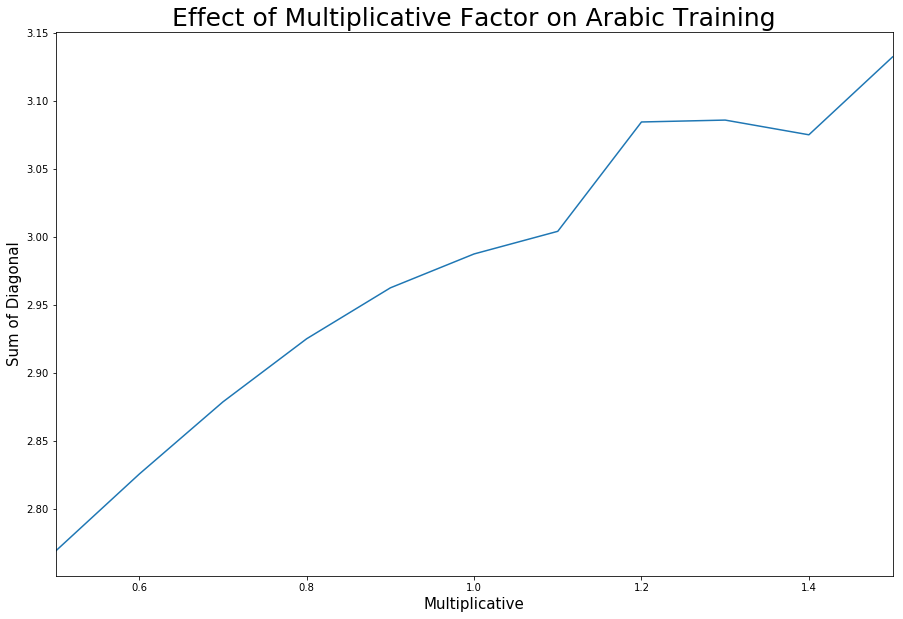
\includegraphics[width=\textwidth,clip]{images/MultiplicativeFactor.png}
\end{figure}
\FloatBarrier

It clearly shows that the higher the factor, the higher the sum of the diagonal i.e. the higher the chance that it stays in a given stage from day to day. The benchmark that we're using though is the one from no training which gets a value of 2.027 which is greater than all of these values thus showing that any level of training gives us more evidence of staying in the same stage. And so, it still seems fairly sensible to stay with our initial assumption of not using a multiplicative factor. The question that we can now ask is whether this trend that training the data on our HMM causes it to prefer staying on the same stage is true more broadly for languages other than Arabic. We look at the main 14 languages mentioned earlier and plot the original sums vs the trained sums.
\FloatBarrier
\begin{figure}[hbtp]\centering
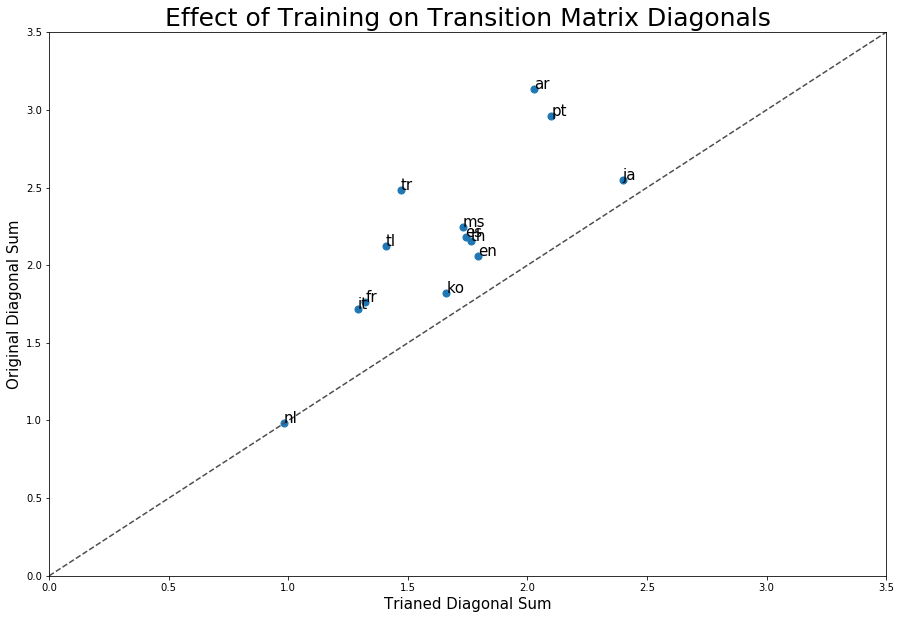
\includegraphics[width=\textwidth,clip]{images/TrainingEffectDiagonals.png}
\end{figure}
\FloatBarrier

We can see that in fact, almost all of them have greater diagonal sums though the amount this varies a lot from Dutch which had no change to Arabic and Portuguese which had around 50\% more. This effect was especially noticeable given that the maximum possible value is 4 if the identity is taken.

\newpage
\section{Answers to Hypotheses}
\subsection{Short-term surge leading to long-term growth}
Our hypothesis was that short-term surges do lead to long-term growth in the language growth rather than just immediately declining. The high results of the diagonal already suggest that this is true since the probability of staying in surge mode after previously being in surge are quite high. However, we choose to make a more detailed approach. We instead want to find the hitting time of state 0 given that we start at state 3. We can define the function $\phi_j = E_j T_0$, the expected time to hit 0 starting at j where our goal is to find $\phi_3$. To solve for $\phi$, we can use the Markov Property to get the following recursion.
\begin{align*}
\phi_j = \begin{cases}
       \quad 1 &\quad j = 0\\
       1+\sum_{k \neq j} A_{j,k}\phi_k &\quad j \neq 0 \\
     \end{cases}
\end{align*}\\
Rewriting this as a matrix problem and solving, we get the following:\\
\begin{align*}
    \begin{bmatrix} \phi_1 \\ \phi_2 \\ \phi_3 \end{bmatrix}  =& \begin{bmatrix} A_{1,1}  & A_{1,2} & A_{1,3} \\ A_{2,1} & A_{2,2} & A_{2,3} \\ A_{3,1} & A_{3,2} & A_{3,3} \end{bmatrix} \begin{bmatrix} \phi_1 \\ \phi_2 \\ \phi_3 \end{bmatrix} + \begin{bmatrix}1+A_{1,0} \\ 1+A_{2,0} \\ 1+A_{3,0}\end{bmatrix}\\\\
\end{align*}
\begin{align*}
    -\begin{bmatrix}1+A_{1,0} \\ 1+A_{2,0} \\ 1+A_{3,0}\end{bmatrix} =& \begin{bmatrix} A_{1,1} - 1 & A_{1,2} & A_{1,3} \\ A_{2,1} & A_{2,2} - 1 & A_{2,3} \\ A_{3,1} & A_{3,2} & A_{3,3} - 1 \end{bmatrix} \begin{bmatrix} \phi_1 \\ \phi_2 \\ \phi_3 \end{bmatrix}\\\\
     \begin{bmatrix} \phi_1 \\ \phi_2 \\ \phi_3 \end{bmatrix} =& -\begin{bmatrix} A_{1,1} - 1 & A_{1,2} & A_{1,3} \\ A_{2,1} & A_{2,2} - 1 & A_{2,3} \\ A_{3,1} & A_{3,2} & A_{3,3} - 1 \end{bmatrix}^{-1} \begin{bmatrix}1+A_{1,0} \\ 1+A_{2,0} \\ 1+A_{3,0}\end{bmatrix}
\end{align*}
We apply this across our 14 languages using the transition matrices attained from the K-means algorithm and get the following table showing our values.
\FloatBarrier
\begin{table}[hbtp]
\begin{center}
\captionof{table}{Hitting Times for Different Languages}
\begin{tabular}{lr}
\toprule
Language &  Expected Hitting Time (in Days) \\
\midrule
en       &    16.765823 \\
ja       &     7.541042 \\
es       &     4.760582 \\
ar       &     2.000000 \\
pt       &    27.183113 \\
ms       &     2.722721 \\
ko       &     2.926538 \\
tr       &    22.625000 \\
th       &     2.000000 \\
fr       &    30.542857 \\
nl       &     2.000000 \\
tl       &     2.335450 \\
it       &     2.110538 \\
\bottomrule
\end{tabular}
\end{center}
\end{table}
\vspace{0.5cm}
\FloatBarrier
From here, we can see that in some languages, the hitting time is fairly large (English, Portuguese,Turkish,French \& Japanese). For these languages, we can clearly see that short-term surges do have long-term impact in that it takes a long time to return to a relative decline though again this could simply imply a slower growth relative to other languages. However for most of the other languages, the expected time to return back to decline is very low which suggests that the surge is very much short-lived and it is quite likely to return back to its original state having been through some decline.
\subsection{Language Similarities}
Our next hypothesis was that there were similarities in growth behaviour between languages that have similar levels of bilingualism. The distance metric we use here to compare growth trends is simply the 'sup-norm' which takes the maximum absolute value across any term in the matrix. This gets us the following (symmetric) table of distances.\\
\begin{table}[hbtp]
\begin{center}
\begin{tabular}{lrrrrrrrrrrrrr}
\toprule
{} &    en &    ja &    es &    ar &    pt &    ms &    ko &    tr &    th &    fr &    nl &    tl &    it \\
\midrule
en &  0.00 &  & & &   &  &   &   &   &  &  &   &   \\
ja &  0.51 &  0.00 &&&&&&&&&&&\\
es &  0.21 &  0.72 &  0.00 &&&&&&&&&&   \\
ar &  0.98 &  0.86 &  0.92 &  0.00 &&&&&&&&& \\
pt &  0.69 &  0.60 &  0.86 &  0.99 &  0.00 &&&&&&&& \\
ms &  0.98 &  0.83 &  0.93 &  0.79 &  0.47 &  0.00 &&&&&&& \\
ko &  0.51 &  0.42 &  0.48 &  0.78 &  0.53 &  0.78 &  0.00 &&&&&& \\
tr &  0.64 &  0.80 &  0.59 &  0.34 &  0.93 &  0.72 &  0.47 &  0.00 &&&&& \\
th &  0.91 &  0.86 &  0.88 &  0.66 &  0.99 &  0.79 &  0.56 &  0.88 &  0.00 &&&& \\
fr &  0.97 &  0.86 &  0.92 &  0.18 &  0.99 &  0.79 &  0.78 &  0.34 &  0.84 &  0.00 &&& \\
nl &  1.00 &  0.89 &  0.96 &  0.74 &  0.99 &  0.79 &  0.78 &  0.96 &  0.35 &  0.92 &  0.00 && \\
tl &  0.79 &  0.68 &  0.76 &  0.53 &  0.78 &  0.56 &  0.59 &  0.75 &  0.44 &  0.71 &  0.44 &  0.00 &   \\
it &  0.98 &  0.86 &  0.93 &  0.19 &  0.99 &  0.79 &  0.78 &  0.34 &  0.85 &  0.12 &  0.93 &  0.72 &  0.00 \\
\bottomrule
\end{tabular}
\end{center}
\end{table}
\FloatBarrier
From here, we can see that there are very few similar pairings. The only ones with a supnorm of less than 0.25 are English-Spanish and the Italian-Arabic-French trio with Turkish not too far at 0.34 from these three. These are quite interesting to note and given that Italian is only the 14th most common language while French is the 11th, we can use Arabic as a clearer proxy language given the larger sample size to work from. The Spanish-English pairing is interesting but not hugely surprising given they're two very well grown languages with similar use patterns. What is interesting is that the pairs that we expected e.g. Japanese, Korean and Thai or Italian and Filipino(tl) are not that similar on an absolute scale. However, Japanese is closer to Korean than any other language and vice-verse and they both have little bilingualism suggesting that there is some similarity to notice here.  We conclude that our hypotheses that language growth over time is related to bilingual use was largely incorrect though the Japanese-Korean relationship may be one to explore more in future studies. One should be cautious though that this data is analysed proportionally and doesn't look at the 'very earliest' stage where bilinguals may have the most effect on language growth.
\subsection{English as a proxy}
In most of the previous literature related to Twitter, English is seen as the base and almost all studies are done in English with the tacit assumption that other languages will act similarly to English. We explicitly question this assumption in this report and look at the effect of using English as our baseline model on the likelihood of observing the different growth patterns in other languages.  The table below shows the log likelihood of the observation of post growths of each model under the trained hidden Markov model \cite{Distancemetric} in English.

\begin{table}[hbtp]
\begin{center}
\captionof{table}{Log Likelihood with English as a base}
\begin{tabular}{lr}
\toprule
 Language &  Log Likelihood \\
\midrule
       en &     2406.709869 \\
       ja &     -590.208024 \\
       es &      925.397334 \\
       ar &     -474.177388 \\
       pt &      413.507636 \\
       ms &    -1400.116965 \\
       ko &    -5426.107175 \\
       tr &   -18392.757059 \\
       th &   -19616.496031 \\
       fr &   -13901.041404 \\
       nl &   -32416.913364 \\
       tl &   -20819.024792 \\
       it &   -13885.483135 \\
\bottomrule
\end{tabular}
\end{center}
\end{table}
\FloatBarrier
\vspace{0.5cm}
As expected, we see English very highly as the model has been designed to optimise for the English data. We also see that it is quite good at explaining the Spanish and Portuguese growth and to a lesser extent Japanese and Arabic but from then onwards, it seems to be very poor. However, what we do see is some relationship between these values and their overall size on Twitter given that these are ordered by overall size. This suggests some relationship between size and similarity as a proxy to English but that largely, most languages are poor proxies to English. This is further emphasised by the analysis in section 6.2.
\newpage
\section{Conclusion}
\subsection{Summary}
We applied the unsupervised clustering techniques and hidden Markov models to our data to help us understand the growth patterns and trends in the data. They have allowed us to make 3 major conclusions:
\begin{enumerate}
\item Short-term surges have clear long-term impacts on some languages (English, Japanese Portuguese, Turkish \& French) while they very often lead to self-adjusting declines in other languages that return the language to pre-surge proportions.
\item The long-term growth patterns of languages aren't very clearly related to the types of bilingual users but there are some pairings of languages that have quite similar growth patterns (e.g. a French-Italian-Arabic grouping and Spanish-English).
\item English often fails to be a good proxy for understanding language growth. In the cases when it is a good proxy, it tends to be for larger languages.
\end{enumerate}
We also found that in general, K-means clustering seemed to work better than Agglomerative Clustering and that the Hidden Markov Model constructed by taking the baseline as the k-means clustering seemed to make growth stages more 'stable' in the sense that they stayed in the same stage more often.
\subsection{Limitations}
There were a number of limitations in our study that prevented the analysis from providing even more insightful conclusions. The first of these was that the we only had proportional data and not absolute data. This was quite limiting because we couldn't measure the actual growth but only the relative growth which artificially forced our measures to be zero-sum in that the growth of some languages caused the decline of others. Another key limitation was that we had a very limited sample of the data and not the entire set. The blocks without data didn't cause huge problems but were a limitation. We were also limited in that we used 'detected' language, which gives us a pretty good picture of the posts at the time but is likely to have some errors. On the positive side, we used the same language detection approach for the full data set, which is much more than any previous study.
\subsection{Potential Extensions}
The analysis focused on the macro growth of languages over time but didn't go into looking at early growth vs later growth to really explore how this changes over time. It could take snapshots at different times and then see if it changes for different languages - this snapshot approach would also have allowed us to look at absolute numbers rather than proportional numbers to account for the changes in the size of data on Twitter over time. We also didn't fully look at the pairs of languages and how they grew together - this is difficult to do because again we have relative numbers and not actual growth and also the clustering techniques similar to the one in this study would be difficult to apply to this problem because we can't really identify which clusters mean what as easily as we could for these. The final question that remains open to explore is that if English isn't a good proxy in terms of language growth - what is a good proxy and how well do these proxy languages apply in a context beyond the macro-level growth of language communities.
\newpage
\begin{thebibliography}{9}

\bibitem{competition3}
Castell\'o, X., Egu\'iluz, V.M., Miguel, M.S., Loureiro-Porto, L., Toivonen, R.I.I.T.T.A., Saram\"aki, J. and Kaski, K., (2008). Modelling language competition: bilingualism and complex social networks. In The Evolution of Language: \textit{Proceedings of the 7th International Conference. Singapore: World Scientific Publishing Co} (pp. 59-66).


\bibitem{Delia}
Delia, Andrea, B., Nicola, P., Bruno, G., Qian, Z., and Mocanu, V. A. (2013). The Twitter of Babel: Mapping World Languages through Microblogging Platforms. \textit{PLoS ONE}, 8(4).

\bibitem{Eleta}
Eleta, I. and Golbeck, J. (2012). Bridging Languages in Social Networks: How Multilingual Users of Twitter Connect Language Communities. \textit{Proceedings of the American Society for Information Science and Technology}, 49(1):1–4.

\bibitem{Garcia}
Garcia-Gavilanes, R., Quercia, D., and Jaimes, A. (2013). Cultural Dimensions in Twitter: Time, Individualism and Power. In \textit{Proceedings of the International AAAI Conference on Web and Social Media, ICWSM 2013}, page 195-204


\bibitem{CLD}
Github, (2013). Compact Language Detection Kit 2. [online] \textit{ Available at: https://github.com/CLD2Owners/cld2 } [Accessed 17 August 2017]



\bibitem{Goncalves}
Gon\c calves, B. and S\'anchez, D. (2014). Crowdsourcing dialect characterization through twitter, \textit{PLoS ONE}, 9(11):e112074.

\bibitem{Gonzalez}
Gonz\'alez-Bail\'on, S., Borge-Holthoefer, J., and Moreno, Y. (2013). Broadcasters and hidden influentials in
online protest diffusion, \textit{American Behavioral Scientist}, doi:10.1177/0002764213479371

\bibitem{Graham}
Graham, M., Hale, S. A., and Gaffney, D. (2014)
Where in the world are you? Geolocation and language identification in Twitter \textit{Professional Geographer} 66(4), pp.568-578.

\bibitem{Halemain}
Hale, S. A. (2014). Global Connectivity and Multilinguals in the Twitter Network, In \textit{Proceedings of the SIGCHI Conference on Human Factors in Computing Systems, CHI 2014}, page 833–842.

\bibitem{HechtEnglish}
Hecht, B. and Gergle, D. (2010). The Tower of Babel Meets Web 2.0: User-Generated Content and Its Applications in a Multilingual Context. \textit{Proceedings of the SIGCHI Conference on Human Factors in Computing Systems, CHI 2014}, pp. 291–300

\bibitem{Hecht}
Hecht, B., Hong, L., Suh, B., and Chi, E. H. (2011).
Tweets from Justin Bieber's heart: The dynamics of the location field in user profiles, In \textit{Proceedings of the 2011 annual conference on Human factors in computing systems, CHI 2011}, page 237–246.


\bibitem{Hong}
Hong, L., Convertino, G., and Chi, E. (2011).
Language matters in Twitter: A large scale study, \textit{International AAAI Conference on Weblogs and Social Media}, page 518–521.

\bibitem{Kim}
Kim, S., Weber, I., Wei, L., and Oh, A. (2014). Sociolinguistic Analysis of Twitter in Multilingual Societies. In \textit{Proceedings of the 25th ACM Conference on Hypertext and Social Media, HT '14}, pages 243–248.

\bibitem{Kwak}
Kwak, H., Lee, C., Park, H., and Moon, S. (2010). What is Twitter, a Social Network or a News Media? WWW '10: \textit{Proceedings of the 19th international conference on World Wide Web}, pages 591–600.

\bibitem{Nguyen1}
Nguyen, D., Doğruöz, A.S., Rosé, C.P., and de Jong, F.M.G. (2016).
Computational Sociolinguistics: A Survey, \textit{Computational Linguistics}, Vol. 42, No. 3, pages 537-593.

\bibitem{Nguyen2}
Nguyen, D., Trieschnigg, D. and Cornips, L. (2015). Audience and the Use of Minority Languages on Twitter. in \textit{Proceedings of the Ninth International Conference on Web and Social Media, ICWSM 2015}, The AAAI Press, pages 666-669.

\bibitem{competition2}
Patriarca, M., Castell\'o, X., Uriarte, J.R., Egu\'iluz, V.M. and San Miguel, M., (2012). Modeling two-language competition dynamics. \textit{Advances in Complex Systems}, 15(03n04), p.1250048.

\bibitem{Oates}
Oates, T., Firoiu, L. and Cohen, P.R., (1999). Clustering time series with hidden markov models and dynamic time warping. In \textit{Proceedings of the IJCAI-99 workshop on neural, symbolic and reinforcement learning methods for sequence learning}, (pp. 17-21). Sweden Stockholm.

\bibitem{Poblete}
Poblete, B., Garcia, R., Mendoza, M., Jaimes, A., (2011). Do all birds tweet the same?: characterizing twitter around the world, \textit{Proceedings of the 20th ACM international conference on Information and knowledge management 2011}, pages 1025-1030.

\bibitem{HMM}
Ritter, A.; Cherry, C.; and Dolan, B. (2010). Unsupervised Modeling
of Twitter Conversations, In \textit{Human Language Technologies: The 2010 Annual Conference of the North American Chapter of the ACL}, pages 172-180


\bibitem{geographies}
Takhteyev, Y., Gruzd, A. and Wellman, B., (2012). Geography of Twitter networks, \textit{Social networks}, 34(1), pp.73-81.

\bibitem{competition}
Vázquez, F., Castell\'o, X. and San Miguel, M., (2010). Agent based models of language competition: macroscopic descriptions and order–disorder transitions. \textit{Journal of Statistical Mechanics: Theory and Experiment} 2010(04), p.P04007.

\bibitem{Weekends}
Yasseri T, Sumi R, Kert\'esz J (2012). Circadian Patterns of Wikipedia Editorial Activity: A Demographic Analysis. \textit{PLoS ONE} 7(1): e30091.

\bibitem{Distancemetric}
Zeng, J. Duan, J. and Wu, C. (2010). A new distance measure for hidden Markov models, \textit{Expert Systems with Applications: An International Journal}, volume 37 n.2, pages 1550-1555


\end{thebibliography}
\newpage
\section{Appendix}
\lstinputlisting{./actual.py}
\end{document}
%\section{References}
%\begin{enumerate}
%\item Hale, S. A. (2014). Global Connectivity and Multilinguals in the Twitter Network. In Proceedings of the SIGCHI Conference on Human Factors in Computing Systems, CHI '14, page 833–842, New York. ACM.
%\item Computer Language Detection Kit - https://github.com/CLD2Owners/cld2

%\end{enumerate}
